% !TEX root = ../thesis-example.tex
%
\section{Restructuring the Code}
\label{sec:impr:enzian}

With the \emph{Chrysalis} system only being a prototype when it was handed to us, code quality had not been a focus so far. To mend this, we were tasked to make way for future expansions and changes to the codebase by generally improving it's architecture. \newline
Since the front-end component \emph{Chrysalis} looked fairly well-built and flexible, we focused on the underlying \emph{Enzian-Yellow}, updating Chrysalis only accordingly when a signature change elsewhere made it necessary.

\begin{figure}[h]
	\centering
	\captionsetup{justification=centering,margin=2cm}
	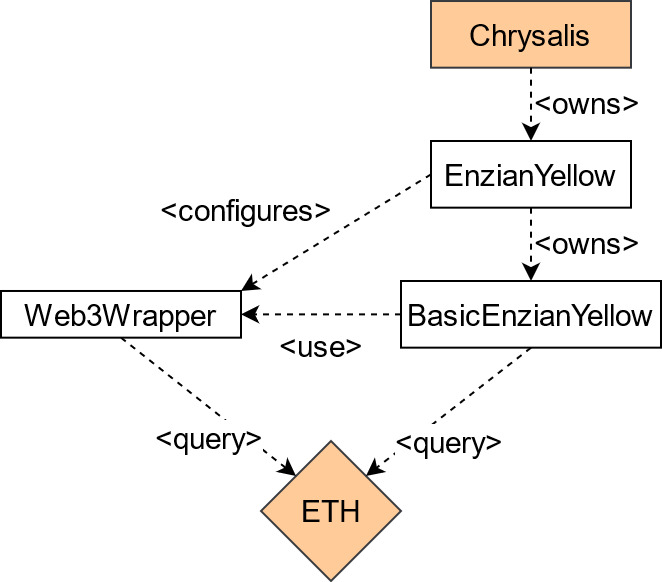
\includegraphics[height=0.5\textwidth]{gfx/enzian-original}
	\caption{Component structure of the original \emph{Enzian-Yellow} Repository. The components marked in orange are not part of Enzian-Yellow, but interact with it.}
	\label{fig:impr:enzian:original}
\end{figure}

As seen in figure \ref{fig:impr:enzian:original}, the architecture of \emph{Enzian-Yellow} consists of three parts, giving us the following understanding:
\begin{itemize}
    \item On the top, the name-giving class \emph{EnzianYellow} is the interface to the applications that use it (like \emph{Chrysalis}): It offers BPM-related methods like creating new processes or tasks and executing the latter, independent of the underlying Blockchain specifics. When constructed, it also instantiates \emph{BasicEnzianYellow} and \emph{Web3Wrapper}.
    \item \emph{BasicEnzianYellow}, as the name might suggest, is a specialization of \emph{EnzianYellow} (though not inheriting from it), offering the same kind of method signature as it's 'parent', but translating these BPM actions into the corresponding Blockchain-transactions. To make these transactions, it sometimes calls the \emph{Web3Wrapper} and sometimes directly queries the \emph{Web3} instance within.
    \item \emph{Web3Wrapper} wraps, as the name indicates, an instance of the class \emph{Web3}, which is the API used to connect and interact with a local \emph{Ethereum} node. It offers functions like deploying contracts, however doesn't fully implement all BPM functionality that \emph{EnzianYellow} offers.
\end{itemize}

\textbf{Tasks} \\[0.2em]
From the given structure, as well as some other observations, the following issues were selected to be solved in this restructuring:
\begin{itemize}
\nopagebreak
    \item The \textbf{Dependencies} in the code does not follow a good and strict hierarchy in the sense of a layer-based architecture, with each layer offering abstraction to and fully satisfying the functional demands of the layer above (Section \ref{sec:impr:enzian:dep}).
    \item In many places, multiple methods with different parameters have the same effect, allowing for \textbf{code duplicates}. Additionally, \textbf{construction} does sometimes not imply object initialization, leaving room for hard-to-explain errors and 'zombie states' (Section \ref{sec:impr:enzian:sig}).
    \item It is not immediately clear, where an \textbf{Expansion}, like adding another Blockchain protocol, would be tied into (Section \ref{sec:impr:enzian:exp}). 
    \item The overall \textbf{Transparency}, especially via log outputs, should be improved (Section \ref{sec:impr:enzian:log}).
\end{itemize}

\subsection{Improving the Dependency Hierarchy}
\label{sec:impr:enzian:dep}

\begin{figure}[h]
	\centering
	\captionsetup{justification=centering,margin=2cm}
	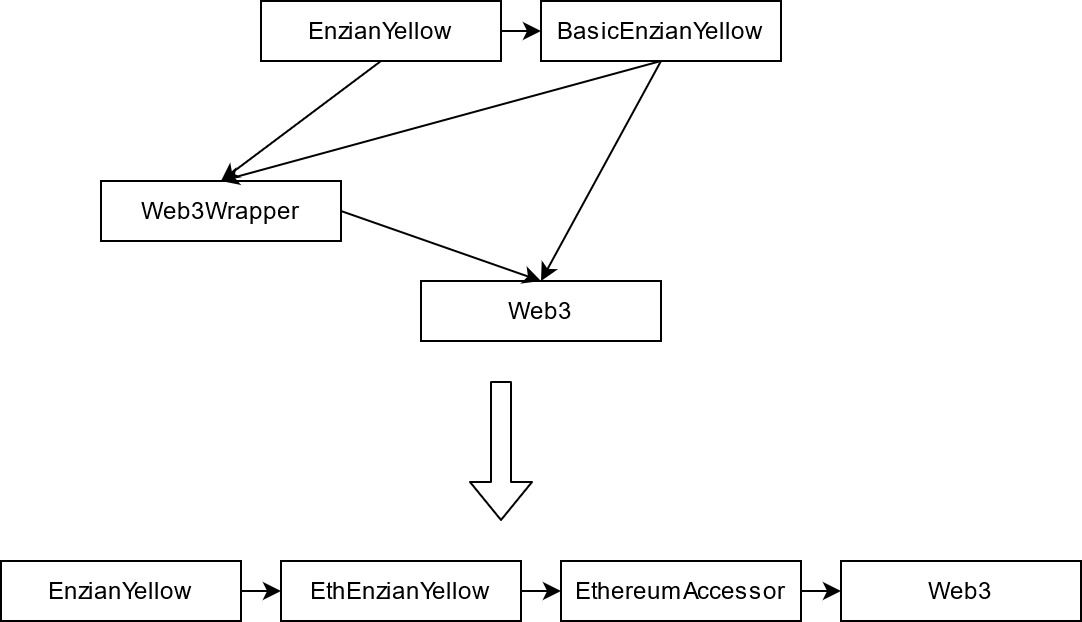
\includegraphics[height=0.5\textwidth]{gfx/enzian-dependencies}
	\caption{The dependency structure of the \emph{Enzian-Yellow} module before and after being reworked, sketched.}
	\label{fig:impr:enzian:dependencies}
\end{figure}

In a fully layered architecture, as we meant to achieve, one layer should never interact with another layer except that above and below. In \emph{Enzian-Yellow} that was not entirely the case. For example, the \emph{Web3Wrapper} object would do interactions with the Blockchain using the contained \emph{Web3} interface, yet the 'parent' object, \emph{BasicEnzianYellow}, would also directly access \emph{Web3}, essentially skipping the wrapper entirely. While this pattern is functional, it is hard to maintain when changes are made to a component, as abstractions of layers are not strict and changes therefore may affect more layers. To achieve a more strict layer-architecture, the following was done:
\begin{itemize}
    \item To fulfill every component's requirements towards lower layers, the first layer underneath was extended to offer all necessary methods, removing the need for layer-skipping.
    \item Code was moved to the specific place where it was meant to be, e.g. actions that required using \emph{Web3} would only be allowed inside the \emph{Web3Wrapper}.
    \item With delegations for every possible method in place, the dependency structure could now be flattened, as shown in figure \ref{fig:impr:enzian:dependencies}.
    \item Finally, in the new structure, a few components were renamed to better reflect their functionality - especially with future expansions in mind. \emph{BasicEnzianYellow} became \emph{EthereumEnzianYellow} and the \emph{Web3Wrapper} became the \emph{EthereumAccessor}.
\end{itemize}

\subsection{Method and Object Signatures}
\label{sec:impr:enzian:sig}

In the prototype system, code was significantly scattered and duplicated, offering the same functionality multiple times with differing parameters, like the example shown in figure \ref{fig:impr:enzian:sig-pre}. As this affects maintainability negatively, we sought to eliminate such redundancies wherever possible.

\begin{figure}[h]
	\centering
	\captionsetup{justification=centering,margin=2cm}
	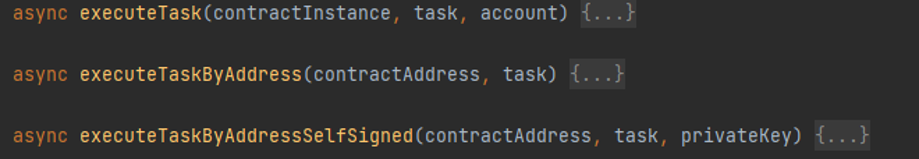
\includegraphics[width=\textwidth]{gfx/enzian-signatures-pre}
	\caption{The 'execute task' method signatures in the original system.}
	\label{fig:impr:enzian:sig-pre}
\end{figure}

Reducing the code scatter boiled down to finding the minimum information with which a method could be executed. In our example case, the \emph{contract instance} argument could be created from the \emph{contract address} - in fact, the instance was always internally created from the address. Additionally, for abstraction purposes, it should not be necessary for the above layers to use such contract instances. Similarly, The \emph{account} and \emph{private key} arguments are equivalent; we opted for only using private keys, as it is a string and therefore more compatible with higher layers, as well.

\begin{figure}[h]
	\centering
	\captionsetup{justification=centering,margin=2cm}
	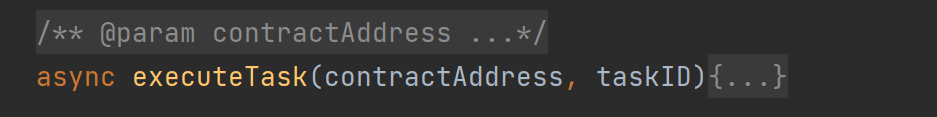
\includegraphics[width=0.7\textwidth]{gfx/enzian-signatures-post}
	\caption{The method signature from figure \ref{fig:impr:enzian:sig-pre} after being merged.}
	\label{fig:impr:enzian:sig-post}
\end{figure}

Additionally, some objects like \emph{Web3Wrapper} would allow being instantiated and configured without being initialized - like connecting to the Blockchain's endpoint, for example. It is generally recommendable to initialize an object immediately when instantiating it, as it could be created successfully while in an invalid state otherwise, leading to potentially hard to understand errors.

With the described changes, the previous example was reduced to the method signature shown in figure \ref{fig:impr:enzian:sig-post}, being a clear improvement, as was done in many other places in the code.

\subsection{Interface for Expansions}
\label{sec:impr:enzian:exp}

With the codebase cleaned up with the methods and principles described in the previous sections, it makes sense to tackle the next design question: How and where should an expansion to the existing system implemented?

\begin{figure}[h]
	\centering
	\captionsetup{justification=centering,margin=2cm}
	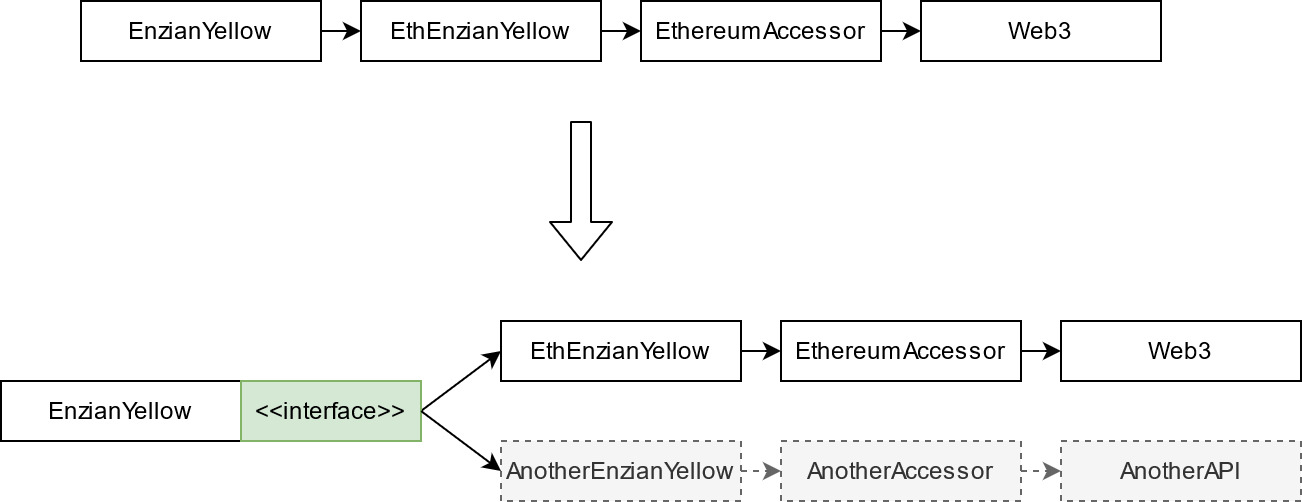
\includegraphics[width=\textwidth]{gfx/enzian-expansion}
	\caption{\emph{Enzian-Yellow}'s Structure before and after introducing an interface for expansion, with a sample expansion sketched in (grey).}
	\label{fig:impr:enzian:expansion}
\end{figure}

As the introduced naming scheme might have already hinted, the perfect way to put an expansion into the current system would be to offer replacements for \emph{EthereumEnzianYellow} that can fill it's signatures. In figure \ref{fig:impr:enzian:expansion} we sketched this as a proper interface, but note that JavaScript as a language does not support such constructs and is weakly typed, meaning that any object with the same method names and signatures may already replace \emph{EthereumEnzianYellow}, no inheritance or implementations needed.

Expanding the \emph{EnzianYellow} module with a new Blockchain of type 'x' is therefore quite simple: One must only make their 'xEnzianYellow' known to the parent class, \emph{EnzianYellow}, and define under which circumstances this new Blockchain application may be used. We opted for a simple constant, passed down to \emph{EnzianYellow} as a string to configure it. If "ethereum" (or, in fact, nothing) is passed for example, \emph{EthereumEnzianYellow} will be selected.

\subsection{Transparency}
\label{sec:impr:enzian:log}



\subsection{Result}
\label{sec:impr:enzian:result}